%%%% 
% This is a template for project reports in the subject DAT620 at the
% Department of Electrical Engineering and Computer Science,
% University of Stavanger.
% 
% The template is based on the ACM conference template 
% it was edited by Leander Jehl and Hein Meling
\documentclass[sigconf]{acmart}

% TODO: edit this somehow
%DON'T CHANGE THIS FILE
%This file sets several properties for the ACM template.
%It is not necessary to change this file.


% Copyright
\setcopyright{none}

% DOI
\acmDOI{}

% ISBN
\acmISBN{}

%Conference
%\acmConference[Copyright: Project in Computer Science (DAT620)]{}{IDE}{UiS}
\acmConference[Project]{}{NLP}{Spring 1401}
\acmBooktitle{}
\copyrightyear{2018}

\newcommand{\supervisors}[1]{\thanks{Supervised by #1}}


%In the preamble file you can include packages and define macros.
\usepackage{xspace}

%Here we define a marco: The \xspace ensures correct spacing, i.e. insert space before next word, but not before period or comma.
\newcommand{\paxos}{\textsc{Paxos}\xspace}

%These packages are needed for the plot in Figure 1. 
\usepackage{tikz}
\usepackage{pgfplots}
\pgfplotsset{compat=newest}



\begin{document}
\title{Natural Language Processing Course Project Report}
%you may use a subtitle
\subtitle{Multi Modal Methods for Emotional Recognition}

\author{Sahel Mesforoosh, Soroush Tabesh, Dorna Dehghani, Amin Kashiri, Fatemeh Tohidian, Seyyed Alireza Mousavizadeh}
\affiliation{Sharif University of Technology, Spring 1401}
%\email{myEmail@stud.uis.no}

\supervisors{Ehsaneddin Asgari}



\begin{abstract}
%The abstract lies in a different file: 
%\textbf{This document serves both as a template and a guideline for your report. You can replace headings and body text with your content. Before you start writing, however, we recommend that you carefully consider the instructions in this document.
%}

%The abstract describes in concise words what you do, why you do it (not
%necessarily in this order), and the main result. The abstract
%has to be self-contained and readable for a person in the
%general area. We suggest to write the abstract first,
%as a means to guide the work, but it should be updated continuously.

Emotions could be recognized in a video by analyzing its text, frames, audio, or a combination of those called "multi-modal methods." In this project, we will propose a few algorithms to combine different features of a video in order to recognize the overall emotion of the scene. Our analysis reveals that this combination in video analysis can result in better emotion recognition models rather than using only one of its aspects.
\end{abstract}

\keywords{NLP, Vision}

\maketitle

%Each section can be placed in a separate file and included by the input command.

\section{Introduction}
\label{sec:introduction}
%
%\noindent
%The introduction is different from the abstract; it should elaborate
%more on the context of the work and other aspects. Generally, you can repeat some
%of the main points also in the introduction, but expand and use different words.
%
%To make your report easier to read, we recommend that you write in first person,
%plural, i.e.~write \textit{we}, even if the report is single author.
%This is also to represent that, even though you are writing this on your own,
%your supervisor and possibly others are contributing ideas, suggestions and
%corrections on your report.
%
%What follows is a possible structure of the introduction.
%Note that the structure can be modified, but the content should be the same.
%Introduction and Abstract should fill at most the first page.

%\paragraph{Context and Motivation} The first few sentences in the introduction
%is typically a brief description providing context for your work, explaining
%the broader domain of the work. This context should lead into the motivation for
%the work by identifying one or more problems.

\paragraph{Context and Motivation} Analyzing and detecting emotions in images and text has been a growing trend in machine learning in recent years. A \textit{video} consists of a number of consecutive images and dialogues or monologues consisting of voice and text. In order to recognize emotions in a video, we can either analyze one of these aspects or combine the result of two or all aspect's. In order to find which features effect the outcome most, we tried different approaches.

%Here is an example from~\cite{zorfu}:

%\textit{Traditional desktop applications, such as word processing, email, and photo management are increasingly moving to server-based deployments. However, moving applications to the cloud can reduce availability because Internet path availability averages only two-nines~\cite{internetPaths}. If a user's application state is isolated on a single server, the availability for that user is limited by the path availability between the user's desktop and that server. Hence, to improve availability, application state must be replicated across multiple servers placed in geographically distributed data centers.}

\paragraph{Research Problem} We considered scripts and frames as the constituents of a video and ignored the sound and tone of expressing speeches, since analyzing those needed additional knowledge which was out of this project's scope. Hence, for the purpose of recognizing the emotions of a video we observed the effect of both video's scripts and its scenes. %TODO summery of models' description 

%\paragraph{Research Problem} This paragraph further restricts the problem introduced in the motivation to the problem you are addressing. 
%Make sure to explain to the reader 
%what you are doing, why it is important, and why it is non-trivial.

%\paragraph{Related Work} 
%\begin{itemize}
%\item Indicated that emotion recognition is significantly better in response to multi-modal versus uni-modal stimuli.~\cite{paulmann2011there} However, this article's results were based on human trials and it did not include any machine learning methods.
%\item Propose a LSTM-based model that enables utterances to capture contextual information from their surroundings in the same video, thus aiding the classification process.~\cite{poria2017context}
%\item This article proposed a context-level inter-modal attention framework for simultaneously predicting the sentiment and expressed emotions of an utterance, evaluated using CMU-MOSEI dataset.~\cite{shenoy2020multilogue}
%\item Proposed a deep neural learning approach based on multiple modalities in which extracted features of an audiovisual data stream are fused in real time for sentiment classification.~\cite{yakaew2021multimodal}
%%TODO: other articles
%\end{itemize}


%\paragraph{Related Work} Next, you have to give a brief overview
%of related work. For a paper like this, anywhere between 2
%and 8 references. Briefly explain what they do. End the paragraph by
%contrasting their work to what you do, to make it precisely clear what
%your contribution is.
%
%\paragraph{Contribution Summary} 
%It can be a good idea to end the introduction with a summary of your contributions as bullet points.
%For example:
%\begin{itemize}
%\item We implement \paxos using brand new technologies.
%\item We evaluate our implementation both in a WAN and LAN environment and show that it is $1.0001\times$ faster than state of the art.
%\end{itemize}
%It is not necessary to have a paragraph at the end of the introduction, that lists the following sections. 


%\section{Literature Review}
%\label{sec:literature}
%Give a short, self-contained summary of necessary background
information. 

For our example if your project is a new \paxos implementation, the background
would be a brief introduction to the consensus problem, the \paxos algorithm,
the system model used by the \paxos algorithm
and common optimizations and relevant variations of that algorithm.

The goal of the background section is to make the paper 
self-contained for an audience as large as possible. As in every
section you start with a very brief overview of the section.
For our example that would be: In this section, we introduce the consensus problem,
the \paxos algorithm and common optimizations of that algorithm.

If you copy a definition from a text book or some other source, you must cite that source. 
See Example~\ref{def:consensus} below. 


%\section{Datasets}
%\label{sec:datasets} 
%There are several datasets for this particular problem, some of which are \textit{MOSI}~\cite{zadeh2016mosi},  \textit{MOSEI}~\cite{zadeh2018multimodal}, and \textit{MSCTD}~\cite{liang2022msctd}. In this section we will introduce these datasets and explore their main features and information.


\subsection{MOSI}
\textit{MOSI} is a dataset of YouTube vlogs (videos of YouTubers expressing their opinion about general subjects) consisting of 2199 video clips from 98 speakers, with a total time of around 2 hours and 36 minutes. These videos vary in quality, distance from camera, lighting, background, etc. There may be more than one speaker in each video. Speakers talk in English and videos are manually transcribed by experts in multiple steps. 
\\
Sentiments in these videos are demonstrated with a linear scale: $-3$ (highly negative), $-2$ (negative), $-1$ (weakly negative), $0$ (neutral), $1$ (weakly positive), $2$ (positive), and $+3$ (highly positive); there was also an "uncertain" choice for not being sure about video's sentiment. Sentiment labeling was performed by online workers with a high approval rate from the Amazon Mechanical Turk website. The distribution of sentiments over the entire dataset is shown in Figure~\ref{fig:MOSIhist}.

\begin{figure}[t]
   \centering
   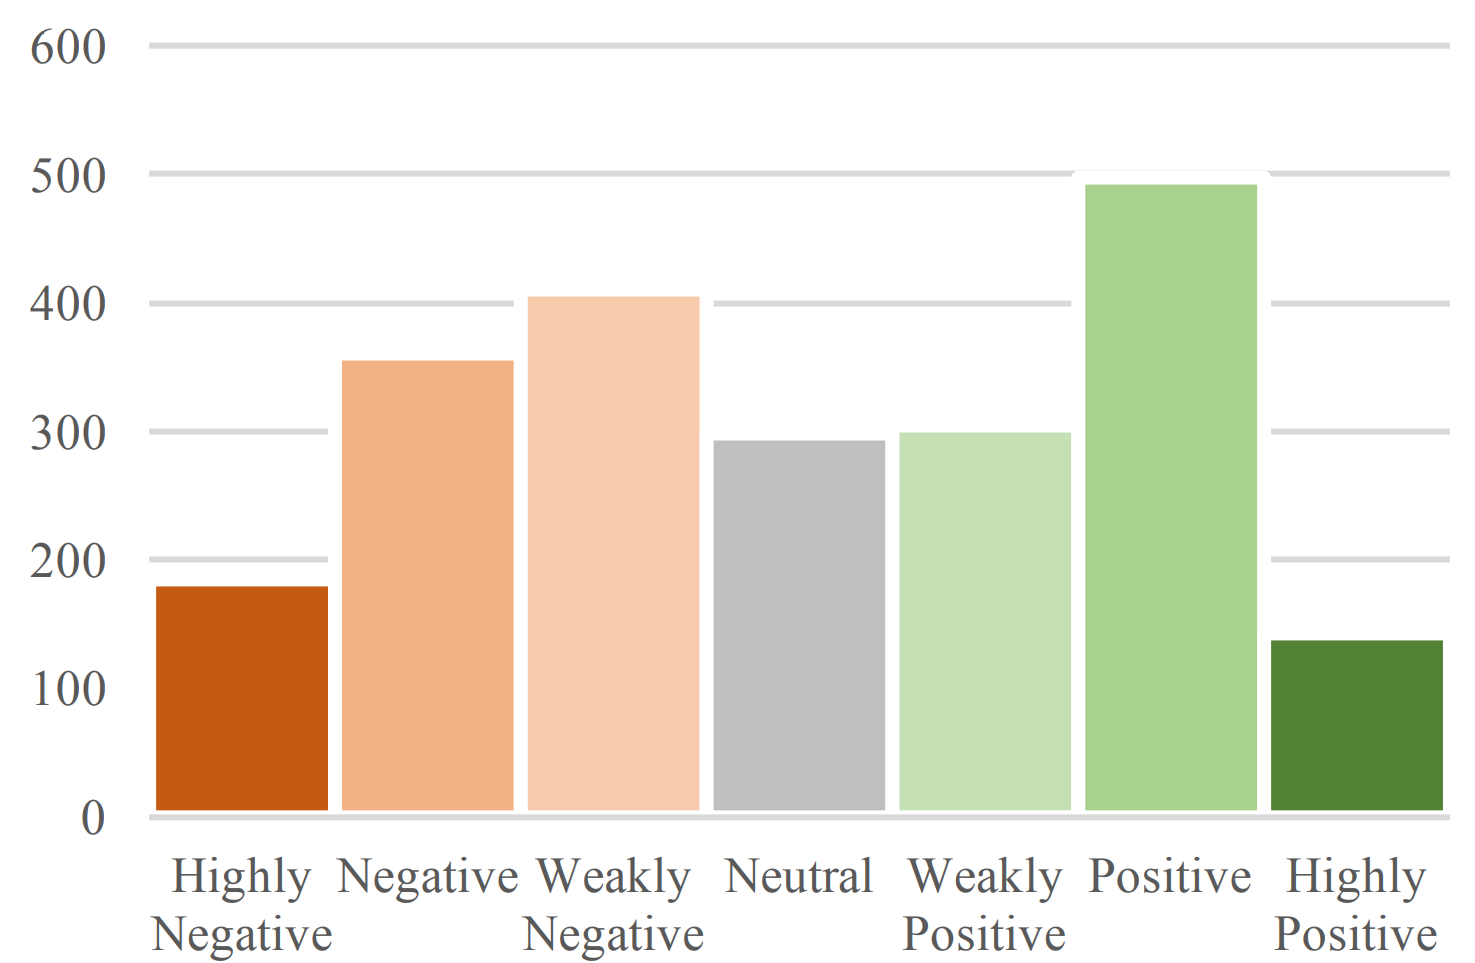
\includegraphics[width=\linewidth]{fig/MOSIhist}
    \caption{Distribution of sentiments over the MOSI dataset, taken from~\cite{zadeh2016mosi}}
    \label{fig:MOSIhist}
\end{figure}

\subsection{MOSEI}
\textit{MOSEI} is the next generation of \textit{MOSI} dataset, a collection of 23453 YouTube video clips from 1000 speakers, with a total time of around 65 hours and 54 minutes. It has the same sentiment labels as \textit{MOSI}, in addition to emotional labels (happiness, sadness, anger, fear, disgust, surprise) labeled by experts. Each video has one speaker and transcribed by its uploader. The distribution of sentiments and emotions over the entire dataset is shown in Figure~\ref{fig:MOSEIhists}. Due to large number of videos contained in this dataset, HPS are needed to process it.

\begin{figure}[t]
	\centering
	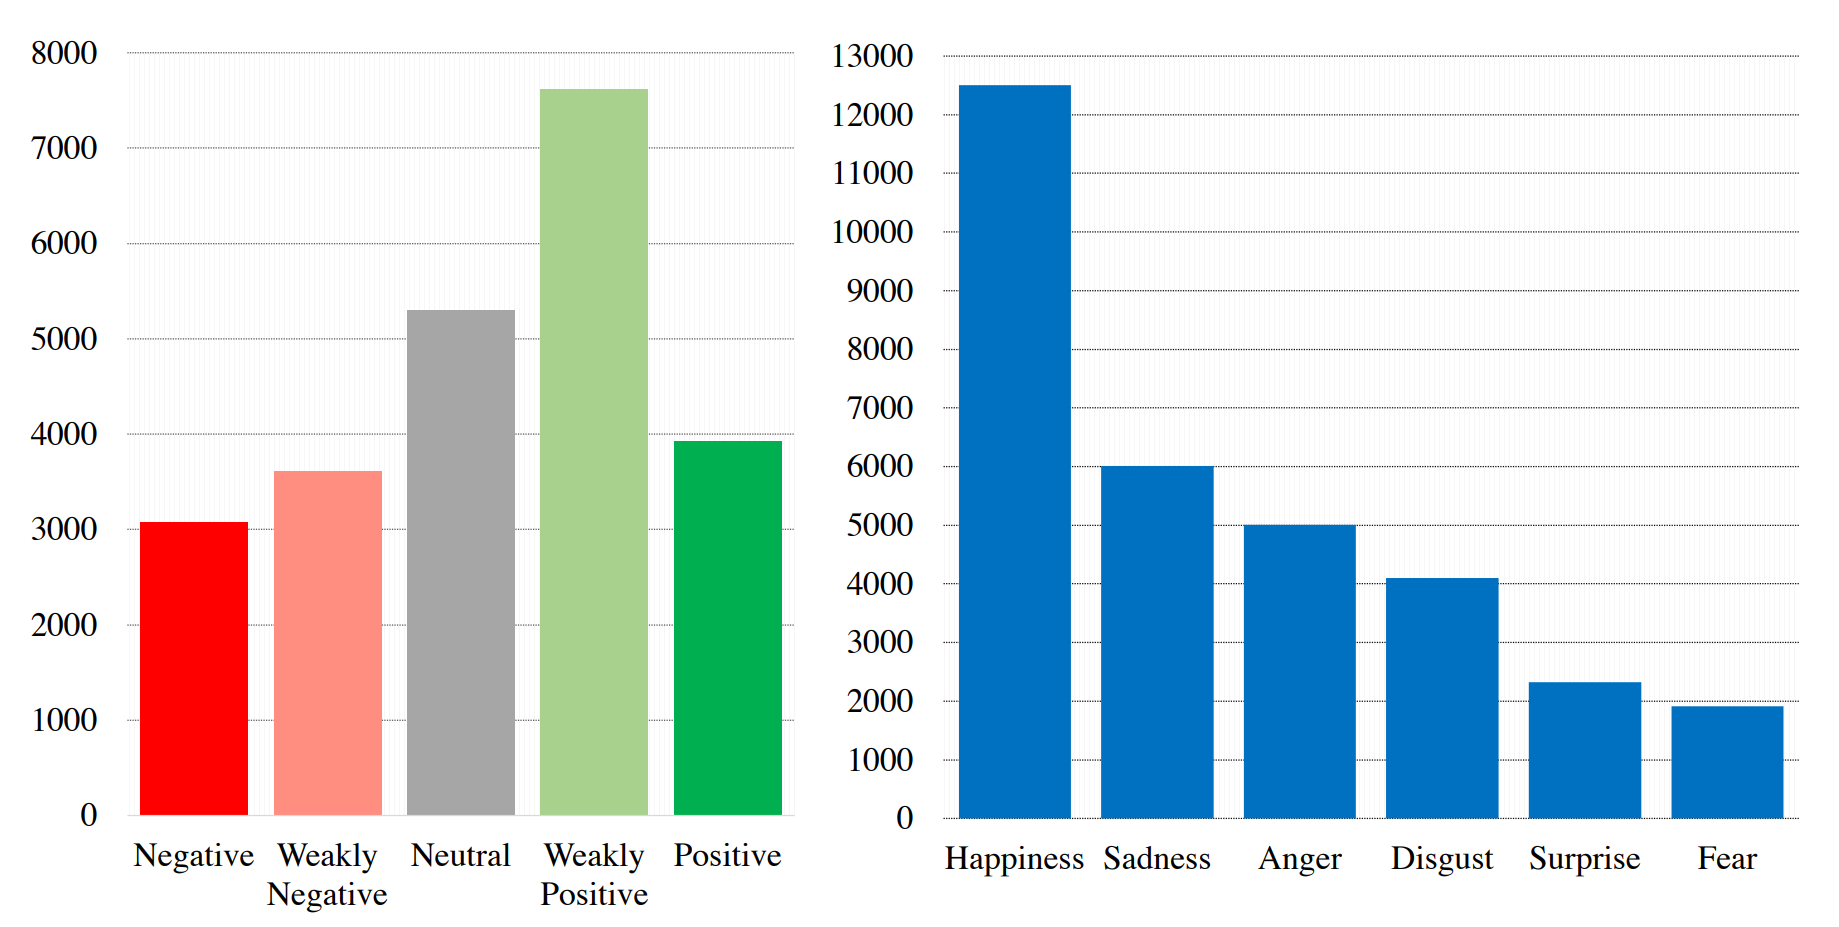
\includegraphics[width=\linewidth]{fig/MOSEIhists}
	\caption{Distribution of sentiments and emotions over the MOSEI dataset, taken from~\cite{zadeh2018multimodal}}
	\label{fig:MOSEIhists}
\end{figure}

\subsection{MSCTD}
Eventually, we decided to use the \textit{MSCTD} dataset. It is a new dataset created in the year 2022 and includes over 17k multi-modal bilingual conversations, consisting of more than 142k English-Chinese and 30k English-German utterance pairs, where each utterance pair corresponds with the associated visual context indicating where it happens. Each visual context of this dataset is a sequence of series or movies images and its dialogues are from OpenViDial dataset~\cite{meng2020openvidial}. In addition, each utterance is annotated with one sentiment label (i.e., positive/neutral/negative). The distribution of sentiments over the entire dataset is shown in Figure~\ref{fig:MSCTDhist}.
\\
This dataset's annotation includes two steps: automatic annotation and then human annotation, for checking and correcting automatic labeling. The size details of the English-German section of the dataset, which we used in our project, can be seen in table \ref{table:MSCTD}.
\\
The advantage of this dataset for us was that we wanted to extract numerous features from each scene. In the previous datasets, we mainly had the face of just one speaker, but here we have the complete scene, which allows us to extract additional features, such as different faces, poses, scene details, etc.

\begin{center}
	\begin{table}[h!]
		\begin{tabular}{||c| c c c||} 
			\hline
			Sentiment & Train & Evaluation & Test \\ [0.5ex] 
			\hline\hline
			Positive & 5483 & 1454 & 1606 \\
			\hline
			Neutral & 6921 & 1764 & 1298 \\
			\hline
			Negative & 7836 & 1845 & 2163 \\ [1ex] 
			\hline
		\end{tabular}
	\caption{Number of each utterance in each section in \textit{MSCTD} dataset}
	\label{table:MSCTD}
	\end{table}
\end{center}


\begin{figure}[t]
	\centering
	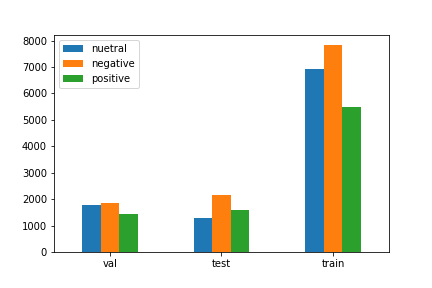
\includegraphics[width=\linewidth]{fig/MSCTDhist}
	\caption{Distribution of sentiments over the MSCTD dataset}
	\label{fig:MSCTDhist}
\end{figure}


\subsection{Other Datasets}
Moreover, there are other datasets that can be used in future works in order to make this project's results more precise. Some of them are:

\begin{enumerate}
	\item \emph{IEMOCAP~\cite{busso2008iemocap}}: Consisted of almost 12 hours of monologues from 10 actors with markers on their faces, heads, and hands, eliciting different emotions during speaking. It needed verification for giving this database which could take a week.
	\item \emph{EmoReact~\cite{nojavanasghari2016emoreact}}: A collected multi-modal basic and complex emotion dataset of children between the ages of four and fourteen years old. It also required up to one-week of verification.
	\item \emph{PATS~\cite{ahuja2020no,ahuja2020style,ginosar2019learning}}: Contains transcribed pose data with aligned audio and transcriptions of 25 speakers of talk shows, lecturers, etc. Using the pose and audio of this dataset can improve our project's outcomes and, therefore, could be considered in future works.
\end{enumerate}

%This section contains some instructions and examples for using \LaTeX.
%
%\subsection{You can add subsections}
%You can use numbered subsections to structure your sections or $\backslash\texttt{paragraph}$ to separate paragraphs with a heading using only a few words, as used in Section~\ref{sec:introduction}.
%
%
%\begin{enumerate}
%	\item\label{item:1} This is an item in an enumeration.
%    \begin{itemize}
%    	\item This is an item of a unnumbered list. In this case, the lists are nested within each other.
%    \end{itemize}
%    \item\label{item:2} The second point in the enumerated list.
%\end{enumerate}
%%
%I can refer to the element of the enumeration above as Point~\ref{item:1}.
%If you refer to numbered items,~e.g. items from a list or figures or sections, always capitalize the name. 
%For example, this is Section~\ref{sec:latex}.
%
%\subsection{Figures}
%You can include figures. You can include files, as done in Figure~\ref{fig:example}. 
%Avoid including jpeg, gif or bmp files since these do not scale nicely. Again Figure~\ref{fig:example} is an example for that.
%
%\begin{figure}[t]
%   \centering
%   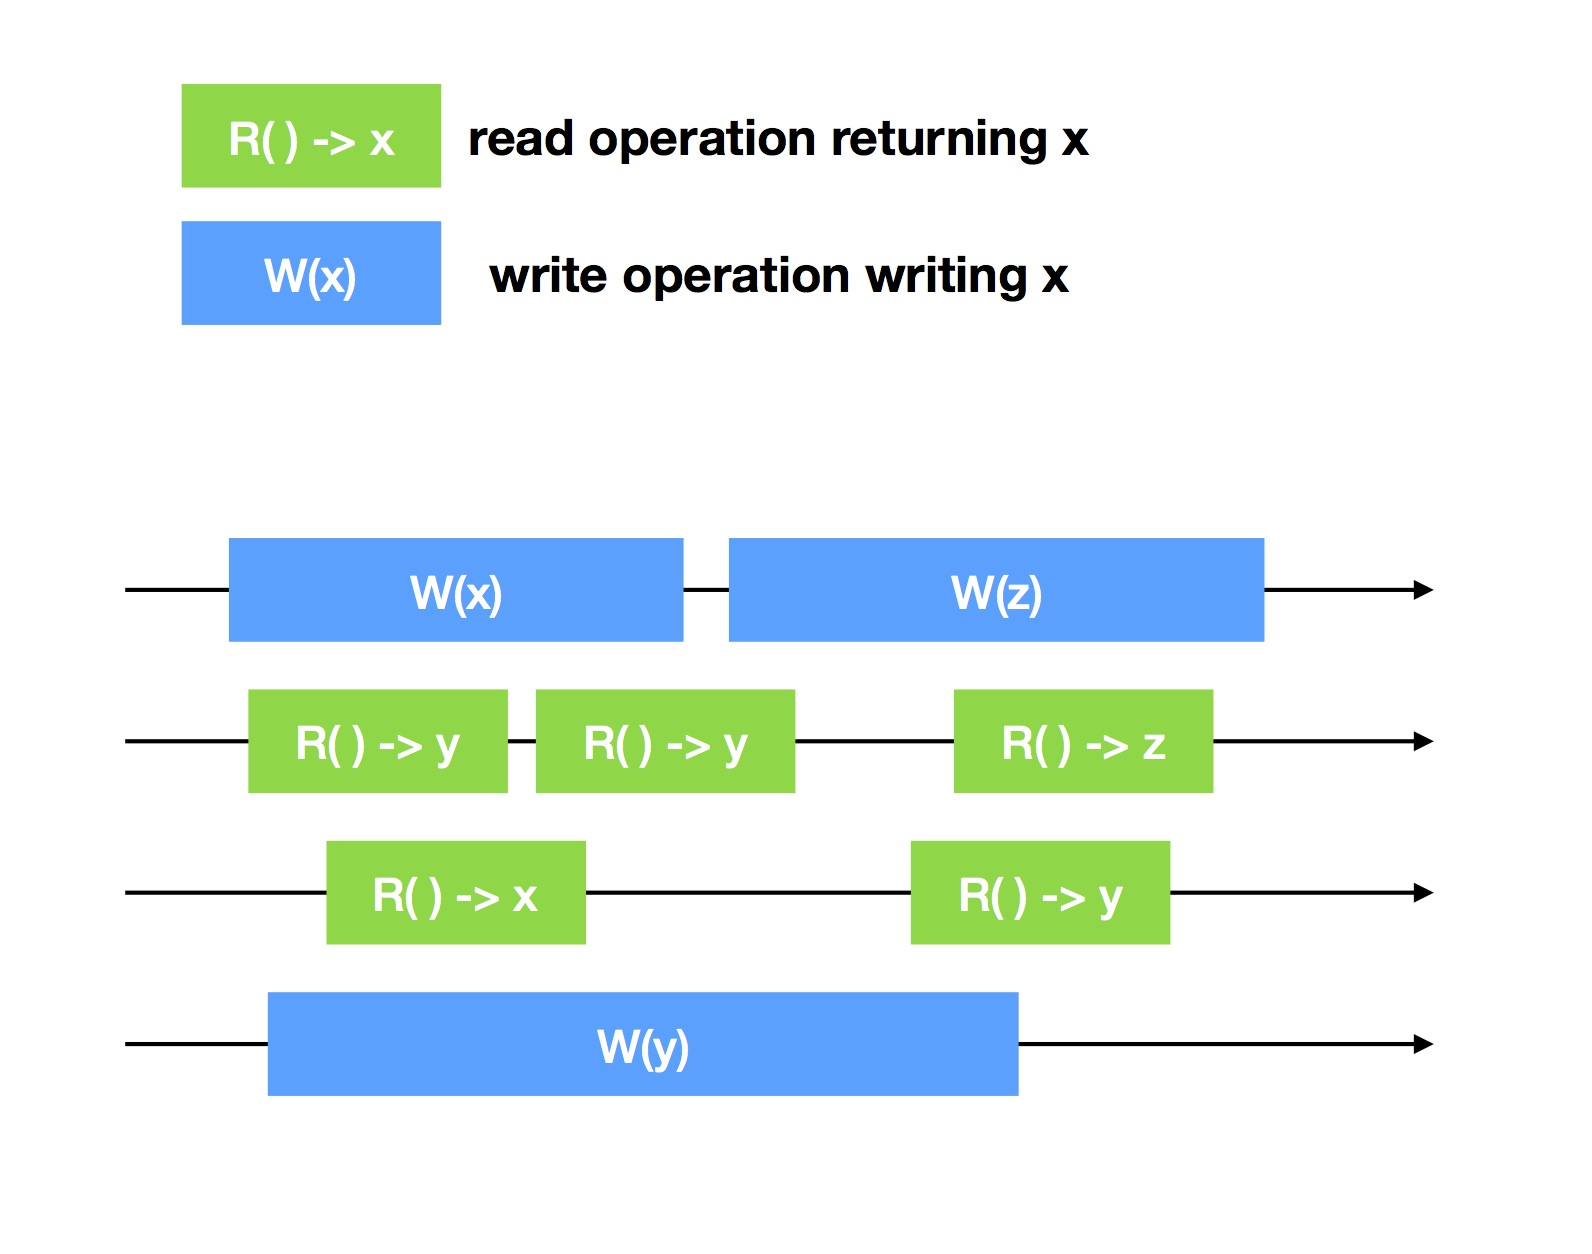
\includegraphics[width=\linewidth]{fig/RegisterOperations}
%    \caption{Figure taken from~\cite{lecture}}
%    \label{fig:example}
%\end{figure}
%
%You can create graphs from your experiment-data using \texttt{pgfplots}.
%See the example in \texttt{tex/evaluation.tex} and documentation \url{http://pgfplots.sourceforge.net/pgfplots.pdf}.
%
%\subsection{Other tips}
%\begin{itemize}
%
%\item Always use the tilde character between the number and unit, e.g. 100~Mbps or 53~ms. The tilde inserts a space, but prevents line break between the number and unit.
%
%\item Never put SI units in italics. 
%
%\item Do differentiate between bits (b) and bytes (B), and between powers of 10~(MB) and 2~(MiB).
%
%\item Avoid things like: "We refer the reader to [42]." That is, don't use citations as nouns.
%\end{itemize}
%
%For further instructions on how to add \textbf{Tables, Algorithms, Theorems see acmguide.pdf}.


%\section{Your Method}
%\label{sec:method}
%Now comes the "beef" of the paper, where you explain what
you did. Again, organize it in paragraphs with titles. As in
every section you start with a very brief overview of the
section. 

This section may vary significantly depending on your topic.
You may also choose to make the different parts individual sections.
Here is a more general structure:

\subsection{Design} Concisely present your design. Focus on novel aspects,
but avoid implementation details. Use pseudo-code and figures to better
explain your design, but also present and explain these in the text.
%
To assist in evaluating your design choices, it may be relevant to describe
several distinct \textit{design alternatives} that can later be compared.

\subsection{Analysis} Argue for the correctness of your design and 
why you expect it to perform better than previous work.
%
If applicable, mention how your design relates to theoretical bounds.

\subsection{Optimization} Explain how you optimized your design and 
adjusted it to specific situations.
%
Generally, as important as the final results is to show
that you took a structured, organized approach to the optimization
and that you explain why you did what you did.
%
Be careful to argue, why your optimization does not break the 
correctness of your design, established above.
%
It is often a good strategy to explain a design or protocol in stepwise refinements,
so as to more easily convince the reader of its correctness. 

\subsection{Implementation} It is not necessary to "explain" your code. 
However, in some cases it may be relevant to highlight 
additional contributions given by your implementation.
Examples for such contributions are:
\begin{itemize}
\item \emph{Abstractions and modules}: If your implementation is nicely separated into interacting
modules with separated responsibilities you could explain this structure,
and why it is good/better than some other alternative structure.
\item \emph{Optimization}: If you spend significant time optimizing your code, e.g.~using profiling tools,
the result of such optimization may be presented as a contribution. In this case, reason, 
why the optimized code works better.
\item \emph{Evaluation framework}: If you implemented a framework or application to evaluate your implementation against existing work, or in a specific scenario, this framework may be presented as a contribution.
\end{itemize}

Make sure to cite all external resources used.

%
%\section{Experimental Evaluation}
%\label{sec:evaluation}
%Here you evaluate your work using experiments. You start
again with a very short summary of the section. The typical
structure follows.

\subsection{Experimental setup}
Specify the context and setup of your experiments. This includes e.g.~what hardware (VMs) you are running on, what operating system these machines are running, how they are connected, ...

Also explain how you generate load for your system and what parameters you used here. The general idea is to include enough information for others to reproduce your experiments. To that end, you should provide a detailed set of instructions for repeating your experiments. These instructions should not be included in the report, but should be provided as part of the source code repository on GitHub, typically as the \texttt{README.md} file, or as Shell scripts or Ansible scripts.

If your experiments give strange or unexpected results, analyze, profile and debug your code. \textbf{Do not simply re-run experiments until they give the expected results.}

Finally, running experiments is very time consuming and you may need to go through multiple rounds of experiment, debugging and optimization. \textbf{Do not delay running experiments until the end of your project period.} 

\subsection{Results}
The results of your experiments. Compare different variants of your design (e.g.~with and without optimizations) or compare performance to other designs or systems. Plots should show the average over multiple runs (at least 10 as a rule of thumb), including error bars, percentiles or min/max values.

Discuss the plot and extract the overall performance. Do not repeat all numbers in the text, but mention relevant differences in numbers, e.g.~our optimization improves throughput by 26\%.
Discuss how the results validate or contradict your assumptions.

Perform experiments to evaluate your system under operating normal conditions, when experiencing failures or attacks, or with different workloads.

Figure~\ref{fig:graph} shows a graph generated with \texttt{pgfplots} from 
experiment data.
\begin{figure}
\begin{tikzpicture}
\begin{axis}[
    xlabel=Throughput ($\times 1000$ Ops/sec),
    ylabel=Latency (ms),
    legend entries={baseline, optimized},
]
%The mockup experiment data is stored in a csv file, and imported here.
\addplot table [x=throughput, y=latency, col sep=comma] {data/data-unoptimized.csv};
\addplot table [x=throughput, y=latency, col sep=comma] {data/data-optimized.csv};
\end{axis}
\end{tikzpicture}
\caption{A graph showing latency and throughput of a baseline and optimized implementation. The axes show latency in milliseconds, and throughput in thousand operations per second. Data is made up.}
\label{fig:graph}
\end{figure}

%
%\section{Conclusion}
%\label {sec:conclusion}
%In this project, we examined a multi-modal model for sentiment recognition in a sequence of frames, in order to evaluate some factors' contribution to this task, i.e. text, face, pose, and scene details. Based on the results, we realized that in sentiment recognition a combination of these factors can lead to better outcomes with higher accuracy and recall.

\paragraph{} This method's results can help label data in other cases. For instance, sentiment recognition in other languages with a small number of data is challenging, but via this model, many data could be classified and prepared for sentiment recognition training.


%Here you need to summarize what you did and why this is
%important. Do not take the abstract and put it in the past
%tense. Remember, now the reader has (hopefully) read the
%paper, so it is a very different situation from the abstract.
%Try to highlight important results and say the things you really
%want to get across such as high-level statements (e.g.,
%we believe that .... is the right approach to .... Even though
%we only considered LAN, the .... technique should be applicable
%....) You can also formulate next steps if you want.
%Be brief.
%
%\section{Citation}
%\label{sec:citation}
%It is important that you correctly refer to sources. 

\begin{itemize}
\item If you describe background, according to some textbook, cite that textbook. \emph{See Example~\ref{def:consensus} below.}
\item If you make a claim about trends in industry or research, add citations to validate the claim. \emph{See Example~\ref{ex:trend} below.}
\item \textbf{Do not copy paste text from any source into your report without citation. It will be considered plagiarism.}
\item Always use the tilde character between the text and the cite command, e.g.:\begin{verbatim}
DBLP~\cite{dplg}
\end{verbatim}
The tilde inserts a space, but prevents line break between the text and citation.
\item For correct citations we recommend that you export bibtex entries from DBLP~\cite{dplg}. 
%@Hein: ACM produces crappy doi-urls for non ACM publications. I do believe that there are few papers that are part of the ACM-DL and not in DBLP.
But make sure to update the bibtex entries to adhere to the following rules.
\end{itemize}

Here are some rules to be followed for your bibliography:

\begin{itemize}
\item Make sure titles are correctly capitalized.

%You can export all nsdi citations from DBLP, accordingly this should not be a problem.
% \item Make sure abbreviations are consistent (e.g., is NSDI spelled out or
% not?) - using the @abbrev function in latex helps here.

\item Make sure there is enough info for a reader to find the document: authors
plus title isn't enough.

\item Don't blindly copy and paste ACM bibtex entries without fixing them:

- they list "New York, NY" as the address field, which means that all ACM
conferences look like they took place there; just delete this, or - better

- replace it with where the conference took place, which is much more
helpful to the reader than the publisher's address

- they have a truly weird idea about how to capitalize conference names;
just correct this (consistently)

* IEEE is equally bad, and uses a partially-inverted form of conference
names.

* Please actually review the bibliography before submitting your paper!
\end{itemize}

%@Leander: Move this to the Latex part:

And while you are at it, please:

\begin{itemize}
\item Add include{mathpmtc} in the main LaTeX file, so you don't have
math stuff in a different font than the main text. 
%We could simply add this to the template if not already done.

\item Always use the tilde character between the number and unit, e.g. 100~Mbps or 53~ms. 
The tilde inserts a space, but prevents line break between the number and unit.

\item Never put SI units in italics. 

\item Do differentiate between bits (b) and bytes (B), and between powers of 10~(MB) and 2~(MiB).

\item Avoid things like: "We refer the reader to [42]." That is, don't use citations as nouns.
\end{itemize}


\begin{example}
\label{def:consensus}
Consensus is a distributed programming abstraction that fulfills the following properties~\cite{aTextbook}:
\begin{description}
\item[Termination]
\item[Validity]
\item[Integrity]
\item[Agreement]
\end{description}
\end{example}

\noindent
\begin{example}
\label{ex:trend} Consensus systems build a fundamental part of todays cloud-computing infrastructure~\cite{spanner,chubby,zookeeper,zookeeperWeb}.
\end{example}



%\section{Further Reading}
%\label{sec:further}
%These multi-modal methods can also be implemented in further languages, other than German, using transcripts and subtitles from those languages.
\\
There have been major successful methods in this field and some of them have been introduced in section~\ref{sec:literature} (Related Work) articles. Adopting their pre-train models and fine-tuning them on our datasets would lead to enhancing the results.
\\
There are different approaches for fixing transformer based model. Using Masked Language Models we can mask embedding of a few scene and use the model to get their embeddings. We can also try other transformer based networks with various loss functions to capture the main problem in the training. 

%Here are some other useful resources: (make these into references instead of links?)
%\begin{itemize}
%\item The co-chairs of the Ninth SOSP prepared some recommendations and valuable lessons in a paper titled \textit{How (and How Not) to Write a Good Systems Paper} \url{https://www.usenix.org/legacy/publications/library/proceedings/dsl97/good_paper.html}
%\item \url{http://gramoli.redbellyblockchain.io/web/doc/talks/researchmethod.pdf}
%\item \url{https://www.doc.ic.ac.uk/~prp/doc/talks/11-prp-paper_writing.pdf}
%\item This template is inspired by a template from Markus P\"uschel~\cite{puschel}.
%
%\end{itemize}

\bibliographystyle{ACM-Reference-Format}
\bibliography{sample-bibliography}

\end{document}
